\subsubsection{Efficiency Achievement}
\label{subsubsec:overall-oop}

\begin{figure}[h]
\vspace{-8pt}
	\centering
		\subfloat[Average $rEFF_{ODP}$] {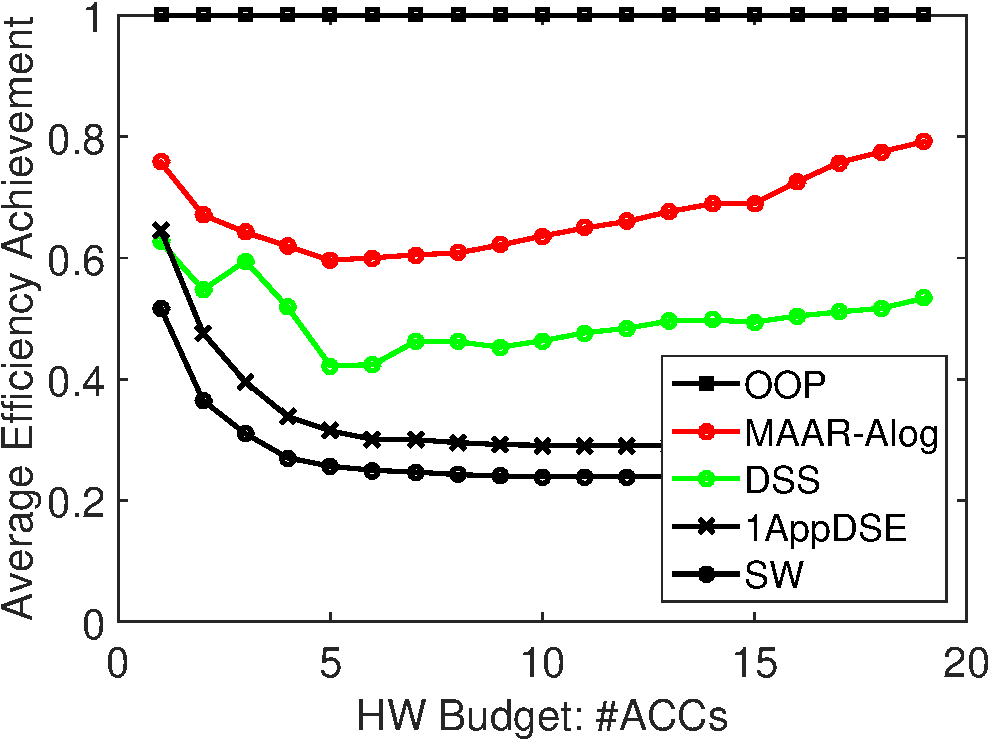
\includegraphics[width=.48\linewidth]{fig/alloop.pdf}\label{fig:alloop}}
		\hfill
		\subfloat[Cumulative Probability (ACCs=12)] {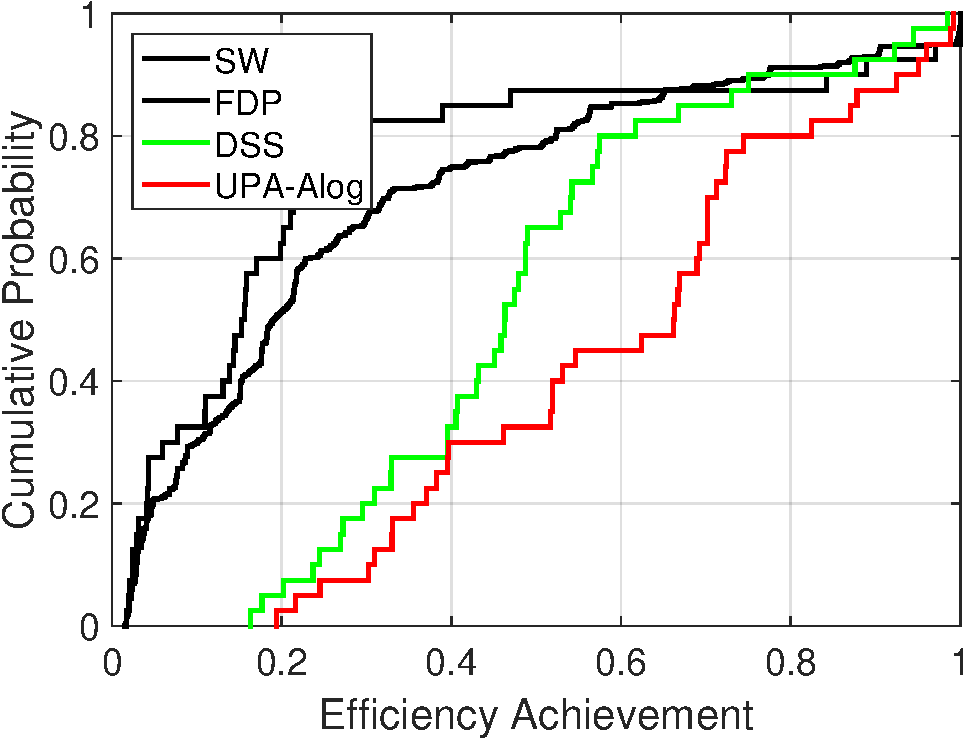
\includegraphics[width=.48\linewidth]{fig/MAARoop12all.pdf}\label{fig:oop12all}}
	\vspace{-8pt}
	\caption{Efficiency Achievement $rEFF_{ODP}$}
	\label{fig:overalloop}
\end{figure}

\figref{fig:alloop} shows the average efficiency achievement ($rEEF_{ODP}$) across all applications of different allocations. 
ODP always achieves 100\% efficiency compared to itself, and is the upper bound.
SW has the lowest efficiency achievement, only reaching about 24\% after ACCs>9. 
UPA-Alog produces a much better efficiency achievement than the other allocations.
On average across the HW budgets, UPA has 1.35 times the efficiency achievement of DSS, and 2.12 times the achievement of FDP.
\figref{fig:alloop} also shows that UPA line is going down when ACCs<5, while it raises after ACCs>5. It means that UPA has a lower improvement speed than ODP when the HW budget is less than 5. However, after this point, UPA improves faster than ODP. As ODP has already accelerated almost all computationally expensive kernels, there are less potential efficiency improvement for ODP.  


\figref{fig:oop12all} is the cumulative probability of efficiency achievement with 12 ACCs budget. Similar to \figref{fig:sw12all}, the line positioned more toward the bottom right has a better efficiency improvement.
ODP is optimal point on the right (i.e. vertical line $x=1$ if drawn) as each application runs on its own dedicated platform.
UPA has a significantly higher achievement than FDP and DSS.
55\% ($1-0.45$ in y-axis) of applications obtain at least 60\% (in x-axis) efficiency of their dedicated optimal platform, while FDP and DSS only have 12.5\% ($1-0.875$) and 10\% ($1-0.9$) of applications respectively achieving the same efficiency.


%Since efficiency achievement is relative to OOP, the plot of DSE can also describe the improvement speed between the DSE and OOP.
%MAAR is decreasing while ACCs<5, and increasing while ACCs>5. This 